\begin{thema}{Β}
Στο σχήμα δίνεται η γραφική παράσταση της $f'$ στο $[0, 6]$.
\begin{center}
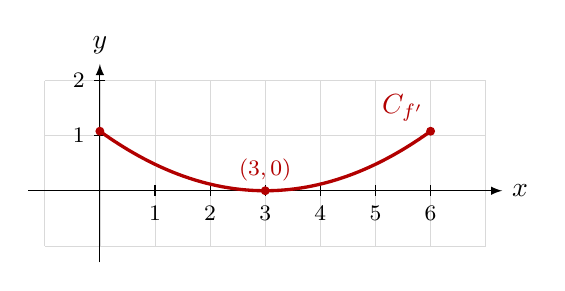
\begin{tikzpicture}[scale=0.7]
  \draw[help lines, gray!30] (-1,-1) grid (7,2);
  \draw[-latex] (-1.3,0) -- (7.3,0) node[right] {$x$};
  \draw[-latex] (0,-1.3) -- (0,2.3) node[above] {$y$};
  \foreach \x in {1,2,3,4,5,6}
    \draw (\x,0.1) -- (\x,-0.1) node[below,font=\footnotesize] {$\x$};
  \foreach \y in {1,2}
    \draw (0.1,\y) -- (-0.1,\y) node[left,font=\footnotesize] {$\y$};
  \draw[very thick, red!70!black, domain=0:6, samples=60] plot (\x, {0.12*(\x-3)*(\x-3)});
  \filldraw[red!70!black] (3,0) circle (2pt) node[above,font=\footnotesize] {$(3,0)$};
  \filldraw[red!70!black] (0,1.08) circle (2pt);
  \filldraw[red!70!black] (6,1.08) circle (2pt);
  \node[red!70!black] at (5.5,1.5) {$C_{f'}$};
\end{tikzpicture}
\end{center}

\begin{erwthma}
  \item Η $f$ παρουσιάζει τοπικό ακρότατο στο $x = 3$; Αιτιολογήστε.
  \item Η $f$ είναι γνησίως αύξουσα ή μη γνησίως αύξουσα στο $[0, 6]$;
  \item Τι κυρτότητα έχει η $f$ εκατέρωθεν του $x = 3$;
  \item Αν $f(0) = 1$, μπορείτε να υπολογίσετε αν $f(6) > 1$;
\end{erwthma}
\end{thema}
